\section{正交曲面坐标系}
在这一节,我们将首先通过我们最熟悉的直角坐标系,把握一般正交曲面坐标系中需要学习的要点,随后以此为基础,推演出柱坐标系和球坐标的相关属性,对比其与直角坐标系的不同。

\begin{Figure}[正交曲面坐标系]
    \begin{FigureSub}[柱坐标系]
        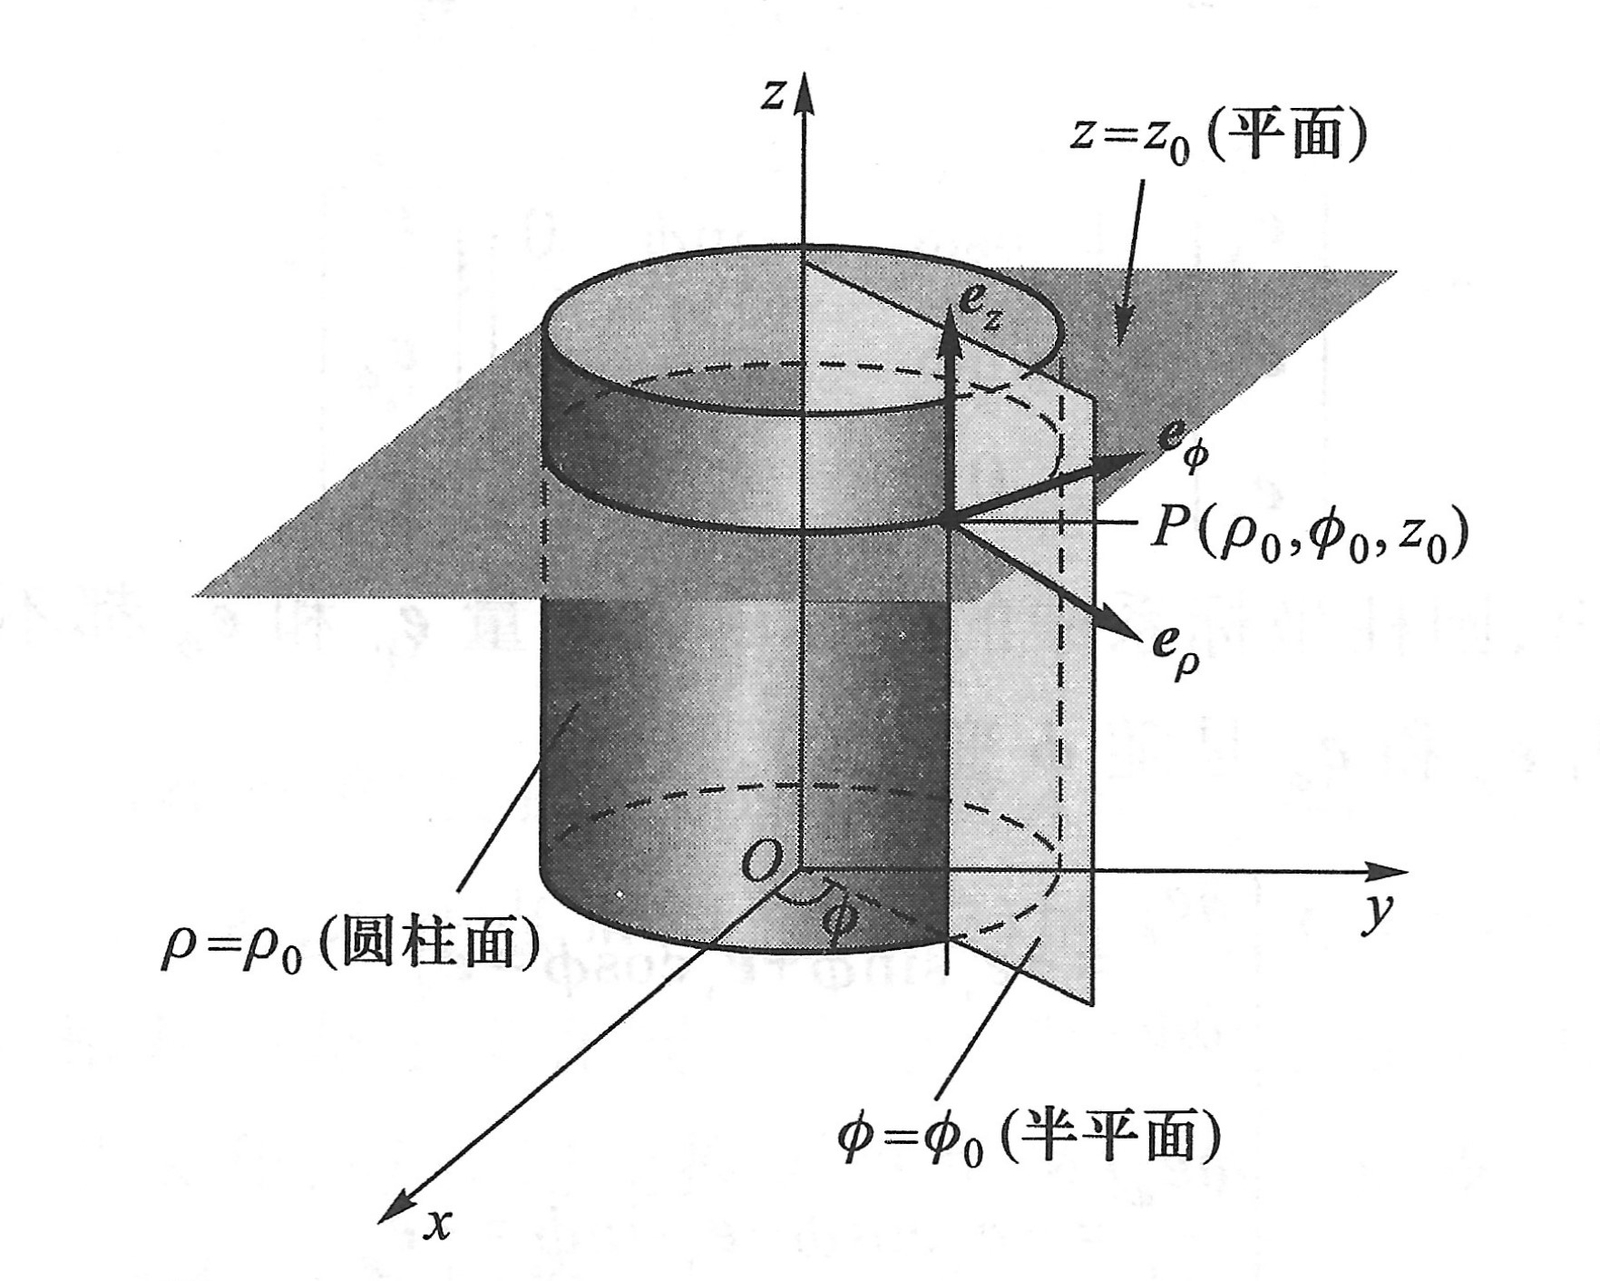
\includegraphics{image/ImageCompress/1.jpg}
    \end{FigureSub}
    \begin{FigureSub}[球坐标系]
        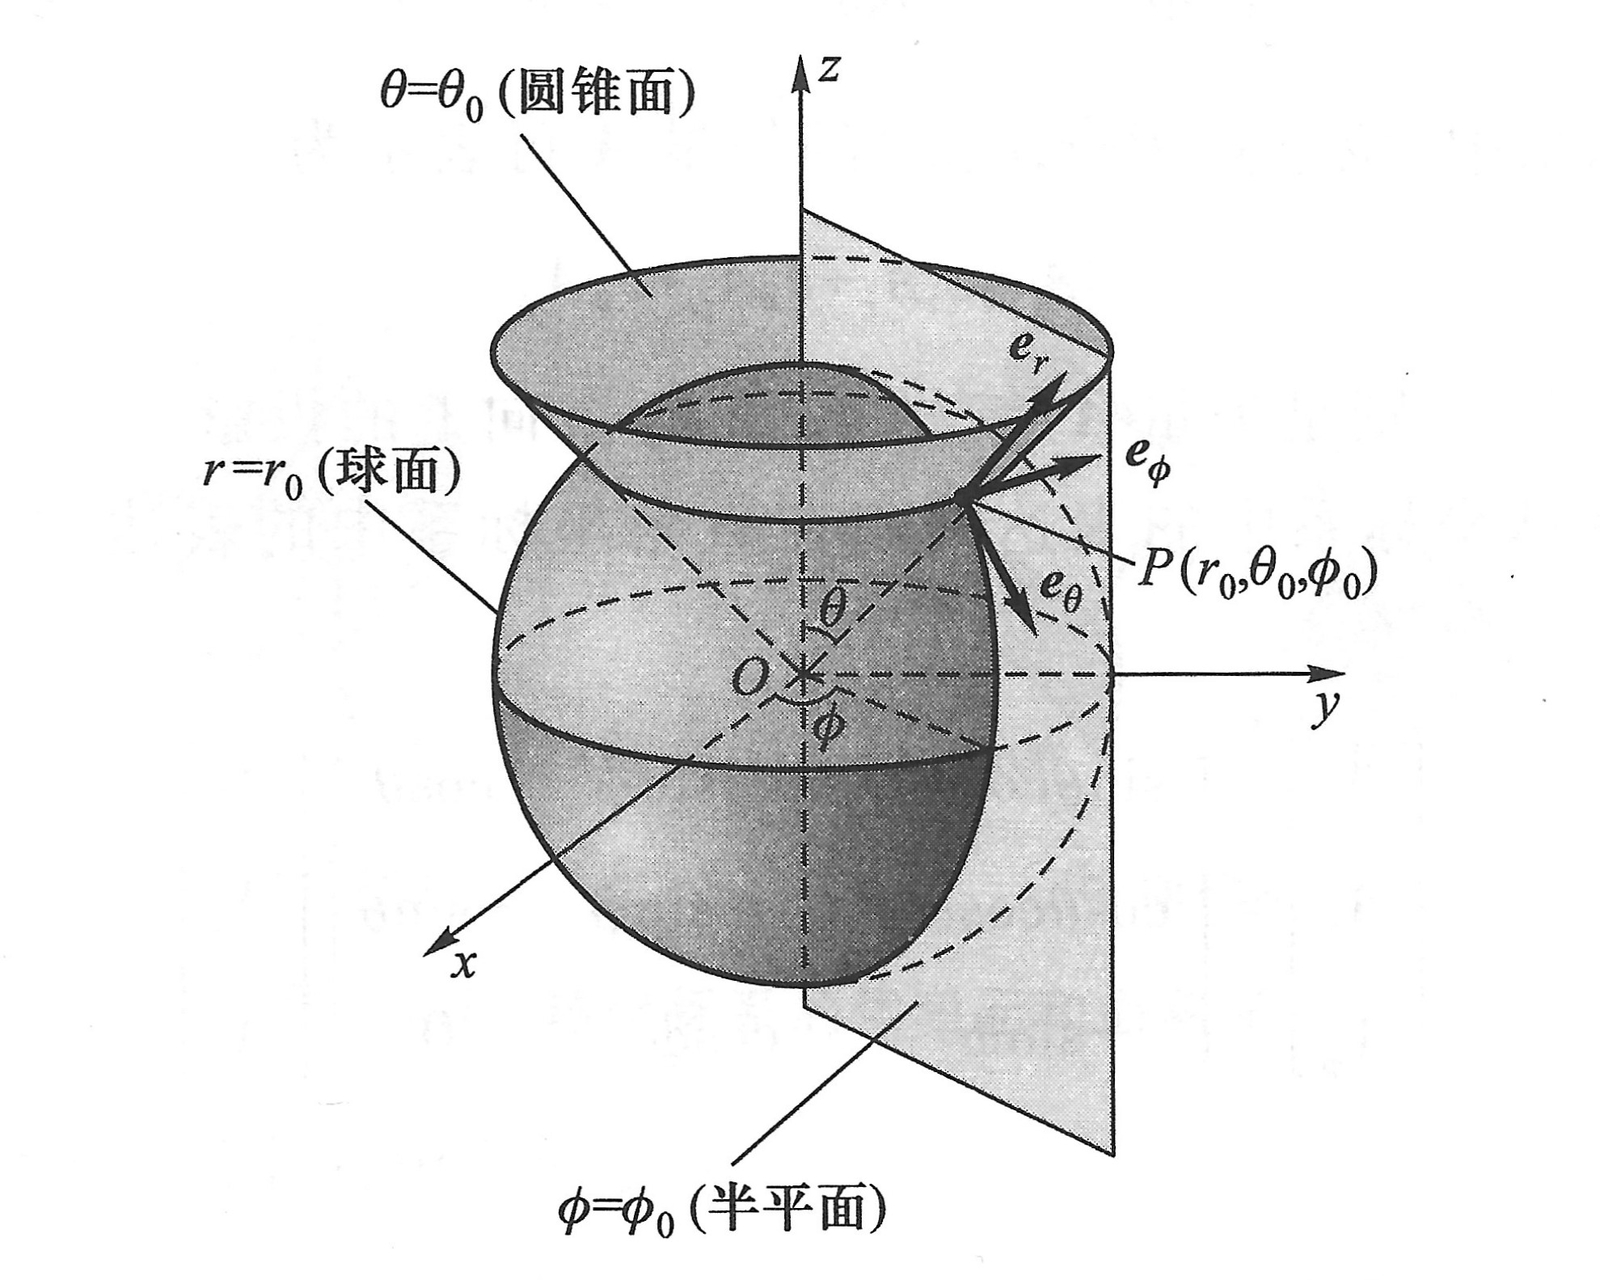
\includegraphics{image/ImageCompress/2.jpg}
    \end{FigureSub}
\end{Figure}

\subsection{直角坐标系}
\begin{BoxDefinition}[直角坐标系]
    直角坐标系中的三个坐标是$(x,y,z)$,它们的变化范围是
    \begin{Equation}&[]
        -\infty<x<\infty\qquad
        -\infty<y<\infty\qquad
        -\infty<z<\infty
    \end{Equation}
\end{BoxDefinition}

直角坐标系的坐标基矢是$\vb*{e}_x,\vb*{e}_y,\vb*{e}_z$,它们是三维空间中三个相互正交的模为$1$的矢量,但事实上,任何一个正交曲面坐标系的单位矢量皆是如此,直角坐标系之所以如此之特别,其实就是因为,\empx{直角坐标系的单位矢量是不随空间位置变化的常矢量},而其他坐标系则未必如此。

直角坐标系中,矢量$\vb*{A}$可以表示为
\begin{Equation}
    \vb*{A}=\vb*{e}_xA_x+\vb*{e}_yA_y+\vb*{e}_zA_z
\end{Equation}
其中$A_x,A_y,A_z$是$\vb*{A}$在$\vb*{e}_x,\vb*{e}_y,\vb*{e}_z$上的投影,实际上,任何坐标系下矢量都可以这样展开为单位矢量的线性组合,但是,\empx{直角坐标系中,矢量在各方向的投影恰好就是矢量的坐标},即这里满足$A_x=x,A_y=y,A_z=z$,而一般的坐标系中,矢量的投影就未必等同于矢量坐标了。

直角坐标系中,具有坐标$(x,y,z)$的矢量,称为\uwave{位置矢量}(Position Vector)。
\begin{BoxFormula}[直角坐标系的位矢]
    直角坐标系中,位置矢量为
    \begin{Equation}&[a]
        \vb*{r}=\vb*{e}_xx+\vb*{e}_yy+\vb*{e}_zz
    \end{Equation}
    其微元矢量为
    \begin{Equation}&[b]
        \dd{\vb*{r}}=\vb*{e}_x\dx+\vb*{e}_y\dy+\vb*{e}_z\dz
    \end{Equation}
\end{BoxFormula}
而由位置矢量的矢量微元,很容易衍生出三个标量微元的概念:长度元、面积元、体积元。

\begin{BoxFormula}[直角坐标系的微元]
    直角坐标系下,长度元为
    \begin{Equation}
        \dd{l_x}=\dx\qquad
        \dd{l_y}=\dy\qquad
        \dd{l_z}=\dz
    \end{Equation}
    直角坐标系下,面积元为
    \begin{Equation}
        \dd{S_x}=\dy\dz\qquad
        \dd{S_y}=\dz\dx\qquad
        \dd{S_z}=\dx\dy
    \end{Equation}
    直角坐标系下,体积元为
    \begin{Equation}
        \dd{V}=\dx\dy\dz
    \end{Equation}
\end{BoxFormula}

\subsection{柱坐标系}
柱坐标系的示意图如\xref{fig:柱坐标系}所示,它标注了等值面和坐标基矢。
\begin{BoxDefinition}[柱坐标系]
    柱坐标系中的三个坐标是$(\rho,\phi,z)$,它们的变化范围是
    \begin{Equation}
        0\leq \rho<\infty\qquad
        0\leq\phi<2\pi\qquad
        -\infty<z<\infty
    \end{Equation}
    柱坐标中,$\rho$表示半径,$\phi$代表相位角,$z$代表高度。

    柱坐标的正变换公式为
    \begin{Equation}
        \rho=\sqrt{x^2+y^2}\qquad
        \phi=\arctan(y/x)\qquad
        z=z
    \end{Equation}
    柱坐标的逆变换公式为
    \begin{Equation}
        x=\rho\cos\phi\qquad
        y=\rho\sin\phi\qquad
        z=z
    \end{Equation}
\end{BoxDefinition}
柱坐标系中,$\rho=\rho_0$为圆柱面,$\phi=\phi_0$为半平面,$z=z_0$为平面。

柱坐标系,或者说一般的正交曲面坐标系中的坐标基矢到底应该怎么定义呢?
\begin{BoxDefinition}[坐标基矢]
    坐标基矢,应当被定义为在空间某点处,各坐标增加的方向。
\end{BoxDefinition}
在直角坐标系中,由于空间各点处坐标$x,y,z$增加的方向都完全相同,因此直角坐标系的坐标基矢是无关空间位置的常数,这是一种幸运,而这种幸运在柱坐标系和球坐标系中不复存在。

由此可见,在柱坐标系和球坐标中,基矢是一个需要仔细考虑一下的概念。

\begin{BoxFormula}[柱坐标系的基矢]*
    柱坐标系的基矢$\vb*{e}_\rho,\vb*{e}_\phi,\vb*{e}_z$的意义分别为
    \begin{itemize}
        \item $\vb*{e}_\rho$代表圆柱面的法线方向,取决于所处位置的相位角$\phi$
        \item $\vb*{e}_\phi$代表圆柱面的切线方向,取决于所处位置的相位角$\phi$
        \item $\vb*{e}_z$代表圆柱的轴方向,是恒定的
    \end{itemize}
    柱坐标基矢的正变换公式为
    \begin{Equation}&[a]
        \begin{pmatrix}
            \vb*{e}_\rho\\
            \vb*{e}_\phi\\
            \vb*{e}_z
        \end{pmatrix}=
        \begin{pmatrix}
            \cos\phi&\sin\phi&0\\
            -\sin\phi&\cos\phi&0\\
            0&0&1\\
        \end{pmatrix}
        \begin{pmatrix}
            \vb*{e}_x\\
            \vb*{e}_y\\
            \vb*{e}_z
        \end{pmatrix}
    \end{Equation}
    柱坐标系的逆变换公式为
    \begin{Equation}&[b]
        \begin{pmatrix}
            \vb*{e}_x\\
            \vb*{e}_y\\
            \vb*{e}_z
        \end{pmatrix}=
        \begin{pmatrix}
            \cos\phi&-\sin\phi&0\\
            \sin\phi&\cos\phi&0\\
            0&0&1\\
        \end{pmatrix}
        \begin{pmatrix}
            \vb*{e}_\rho\\
            \vb*{e}_\phi\\
            \vb*{e}_z
        \end{pmatrix}
    \end{Equation}
    应注意,柱坐标系中$\vb*{e}_\rho,\vb*{e}_\phi$并非常矢量,故
    \begin{Equation}&[c]
        \qquad\qquad
        \pdv{(\vb*{e}_\rho,\vb*{e}_\phi,\vb*{e}_z)}{(\rho,\phi,z)}=
        \begin{pmatrix}
            \pdv*{\vb*{e}_\rho}{\rho}&
            \pdv*{\vb*{e}_\rho}{\phi}&
            \pdv*{\vb*{e}_\rho}{z}\\
            \pdv*{\vb*{e}_\phi}{\rho}&
            \pdv*{\vb*{e}_\phi}{\phi}&
            \pdv*{\vb*{e}_\phi}{z}\\
            \pdv*{\vb*{e}_z}{\rho}&
            \pdv*{\vb*{e}_z}{\phi}&
            \pdv*{\vb*{e}_z}{z}\\
        \end{pmatrix}
        =
        \begin{pmatrix}
            0&\vb*{e}_\phi&0\\
            0&-\vb*{e}_\rho&0\\
            0&0&0
        \end{pmatrix}
        \qquad\qquad
    \end{Equation}
    这很合理,法向的偏导是切向,切向的偏导是法向。
\end{BoxFormula}

柱坐标系下,矢量$\vb*{A}$同样可以表示为
\begin{Equation}[柱坐标的矢量表示]
    \vb*{A}=\vb*{e}_\rho A_\rho+\vb*{e}_\phi A_\phi+\vb*{e}_zA_z
\end{Equation}
这里$A_\rho,A_\phi,A_z$是矢量$\vb*{A}$的投影,但与直角坐标系中不同的是,这里投影$(A_\rho,A_\phi,A_z)$与坐标$(\rho,\phi,z)$并不相同,要将投影$(A_\rho,A_\phi,A_z)$转换为坐标$\rho,\phi,z$,需要两步
\begin{enumerate}
    \item 将$(A_\rho,A_\phi,A_z)$转化为$(A_x,A_y,A_z)$,两者的转换关系与两者基矢的转换关系,即\fancyref{fml:柱坐标系的基矢}给出的$(\vb*{e}_\rho,\vb*{e}_\phi,e_z)$和$(\vb*{e}_x,\vb*{e}_y,\vb*{e}_z)$间的转换关系是完全相同的。
    \item 将$(A_x,A_y,A_z)=(x,y,z)$转化为$(\rho,\phi,z)$,运用\fancyref{def:柱坐标系}。
\end{enumerate}
这样一来,就有
\begin{Equation}
    \begin{pmatrix}
        A_\rho\\
        A_\phi\\
        A_z
    \end{pmatrix}=
    \begin{pmatrix}
        \cos\phi&\sin\phi&0\\
        -\sin\phi&\cos\phi&0\\
        0&0&1
    \end{pmatrix}
    \begin{pmatrix}
        \rho\cos\phi\\
        \rho\sin\phi\\
        z
    \end{pmatrix}
\end{Equation}
柱坐标系中,由于$\vb*{e}_\rho,\vb*{e}_\phi$均会随$\phi$变化的,因此以\xref{eq:柱坐标的矢量表示}方式表示的两个矢量$\vb*{A}_1,\vb*{A}_2$是无法像直角坐标系那样直接进行加法、点积、叉积运算的,除非,它们的相位角$\phi$是相同的。

柱坐标系中,位置矢量的表示也有了很大的变化。
\begin{BoxFormula}[柱坐标系的位矢]
    柱坐标系中,位置矢量为
    \begin{Equation}&[a]
        \vb*{r}=\vb*{e}_\rho\rho+\vb*{e}_zz
    \end{Equation}
    其微元矢量为
    \begin{Equation}&[b]
        \dd{\vb*{r}}=\vb*{e}_\rho\dd{\rho}+\vb*{e}_\phi\rho\dd{\phi}+\vb*{e}_z\dd{z}
    \end{Equation}
\end{BoxFormula}
\begin{Proof}
    这里\xrefpeq{a}是不难理解的,关键在于$\vb*{e}_\rho$是圆心指向圆周上点的单位矢量
    \begin{Equation}&[1]
        \vb*{r}=\vb*{e}_\rho\rho+\vb*{e}_zz
    \end{Equation}
    接下来,对其求微分
    \begin{Equation}&[2]
        \dd{\vb*{r}}=\dd{(\vb*{e}_\rho\rho)}+\dd{(\vb*{e}_zz)}
    \end{Equation}
    应用乘积法则
    \begin{Equation}
        \dd{\vb*{r}}=\vb*{e}_\rho\dd{\rho}+\rho\dd{\vb*{e}_\rho}+\vb*{e}_z\dd{z}+z\dd{\vb*{e}_z}
    \end{Equation}
    应用\fancyref{fml:柱坐标系的基矢}中的\xrefpeq[柱坐标系的基矢]{c},注意到
    \begin{Equation}
        \dd{\vb*{e}_\rho}=\vb*{e}_\phi\dd{\phi}\qquad
        \dd{\vb*{e}_z}=0
    \end{Equation}
    因此
    \begin{Equation}*
        \dd{\vb*{r}}=\vb*{e}_\rho\dd{\rho}+\vb*{e}_\phi\rho\dd{\phi}+\vb*{e}_z\dd{z}\qedhere
    \end{Equation}
\end{Proof}

\begin{BoxFormula}[柱坐标系的微元]
    柱坐标系下,长度元为
    \begin{Equation}
        \dd{l_\rho}=\dd{\rho}\qquad
        \dd{l_\phi}=\rho\dd{\phi}\qquad
        \dd{l_z}=\dz
    \end{Equation}
    柱坐标系下,面积元为
    \begin{Equation}
        \dd{S_\rho}=\rho\dd{\phi}\dz\qquad
        \dd{S_\phi}=\dd{z}\dd{\rho}\qquad
        \dd{S_z}=\rho\dd{\rho}\dd{\phi}
    \end{Equation}
    柱坐标系下,体积元为
    \begin{Equation}
        \dd{V}=\rho\dd{\rho}\dd{\phi}\dd{z}
    \end{Equation}
\end{BoxFormula}

\subsection{球坐标系}
球坐标系的示意图如\xref{fig:球坐标系}所示,它标注了等值面和坐标基矢。
\begin{BoxDefinition}[球坐标系]
    球坐标系中的三个坐标是$(r,\theta,\phi)$,它们的变化范围是
    \begin{Equation}
        0\leq r<\infty\qquad
        0\leq\theta\leq\pi\qquad
        0\leq\phi<2\pi
    \end{Equation}
    球坐标中,$r$表示半径,$\theta$代表天顶角(纬度),$\phi$代表方位角(经度)。

    球坐标的正变换公式为
    \begin{Equation}
        \qquad
        \rho=\sqrt{x^2+y^2+z^2}\qquad
        \theta=\arctan (y/\sqrt{x^2+y^2+z^2})\qquad
        \phi=\arctan(y/x)
        \qquad
    \end{Equation}
    球坐标的逆变换公式为
    \begin{Equation}
        x=r\sin\theta\cos\phi\qquad
        y=r\sin\theta\sin\phi\qquad
        z=r\cos\theta
    \end{Equation}
\end{BoxDefinition}
球坐标系中,$r=r_0$为球面,$\theta=\theta_0$为圆锥面,$\phi=\phi_0$为半平面。

球坐标系下的基矢同样可以用直角坐标的基矢表示
\begin{BoxFormula}[球坐标系的基矢]*
    球坐标系的基矢$\vb*{e}_r,\vb*{e}_\theta,\vb*{e}_\phi$的意义分别为
    \begin{itemize}
        \item $\vb*{e}_r$代表球面的法线方向,取决于所处位置的$\theta,\phi$
        \item $\vb*{e}_\theta$代表球面上,沿纬度的切线方向,取决于所处位置的$\theta,\phi$
        \item $\vb*{e}_\phi$代表球面上,沿经度的切线方向,取决于所处位置的$\theta,\phi$
    \end{itemize}
    球坐标基矢的正变换公式为
    \begin{Equation}&[a]
        \begin{pmatrix}
            \vb*{e}_r\\
            \vb*{e}_\theta\\
            \vb*{e}_\phi
        \end{pmatrix}=
        \begin{pmatrix}
            \sin\theta\cos\phi&
            \sin\theta\sin\phi&
            \cos\theta\\
            \cos\theta\cos\phi&
            \cos\theta\sin\phi&
            -\sin\theta\\
            -\sin\phi&
            \cos\phi&
            0\\
        \end{pmatrix}
        \begin{pmatrix}
            \vb*{e}_x\\
            \vb*{e}_y\\
            \vb*{e}_z
        \end{pmatrix}
    \end{Equation}
    球坐标系的逆变换公式为
    \begin{Equation}&[b]
        \begin{pmatrix}
            \vb*{e}_x\\
            \vb*{e}_y\\
            \vb*{e}_z
        \end{pmatrix}=
        \begin{pmatrix}
            \sin\theta\cos\phi&
            \cos\theta\cos\phi&
            -\sin\phi\\
            \sin\theta\sin\phi&
            \cos\theta\sin\phi&
            \cos\phi\\
            \cos\theta&
            -\sin\theta&
            0\\
        \end{pmatrix}
        \begin{pmatrix}
            \vb*{e}_r\\
            \vb*{e}_\theta\\
            \vb*{e}_\phi
        \end{pmatrix}
    \end{Equation}
    应注意,球坐标系中$\vb*{e}_r,\vb*{e}_\theta,\vb*{e}_\phi$均非常矢量,故
    \begin{Equation}&[c]
        \pdv{(\vb*{e}_r,\vb*{e}_\theta,\vb*{e}_\phi)}{(r,\theta,\phi)}=
        \begin{pmatrix}
            \pdv*{\vb*{e}_r}{r}&
            \pdv*{\vb*{e}_r}{\theta}&
            \pdv*{\vb*{e}_r}{\phi}\\
            \pdv*{\vb*{e}_\theta}{r}&
            \pdv*{\vb*{e}_\theta}{\theta}&
            \pdv*{\vb*{e}_\theta}{\phi}\\
            \pdv*{\vb*{e}_\phi}{r}&
            \pdv*{\vb*{e}_\phi}{\theta}&
            \pdv*{\vb*{e}_\phi}{\phi}\\
        \end{pmatrix}
        =
        \begin{pmatrix}
            0&\vb*{e}_\theta&\vb*{e}_\phi\sin\theta\\
            0&-\vb*{e}_r&\vb*{e}_\phi\cos\theta\\
            0&0&-\vb*{e}_r\sin\theta-\vb*{e}_\phi\cos\theta
        \end{pmatrix}
    \end{Equation}
\end{BoxFormula}
通过\xref{fml:柱坐标系的基矢}和\xref{fml:球坐标系的基矢}可以注意到,基矢的正变换和逆变换的矩阵,互为转置矩阵。\footnote{哈哈,考试可以少记一点了(回想起固体物理考前背答案的痛苦了)。}

球坐标系下,矢量$\vb*{A}$仍然可以表示为
\begin{Equation}[柱坐标的矢量表示]
    \vb*{A}=\vb*{e}_r A_r+\vb*{e}_\theta A_\theta+\vb*{e}_\phi A_\phi
\end{Equation}
这里$A_r,A_\theta,A_\phi$是矢量$\vb*{A}$的投影,它们可以这样由$(r,\theta,\phi)$计算
\begin{Equation}
    \begin{pmatrix}
        A_r\\
        A_\theta\\
        A_\phi
    \end{pmatrix}=
    \begin{pmatrix}
        \sin\theta\cos\phi&
        \sin\theta\sin\phi&
        \cos\theta\\
        \cos\theta\cos\phi&
        \cos\theta\sin\phi&
        -\sin\theta\\
        -\sin\phi&
        \cos\phi&
        0\\
    \end{pmatrix}
    \begin{pmatrix}
        r\sin\theta\cos\phi\\
        r\sin\theta\sin\phi\\
        r\cos\theta
    \end{pmatrix}
\end{Equation}
球坐标系中,只有当$\theta,\phi$均相同时,矢量间才能直接进行计算。

球坐标系中,位矢的形式反而更简单了

\begin{BoxFormula}[球坐标系的位矢]
    球坐标系中,位置矢量为
    \begin{Equation}&[a]
        \vb*{r}=\vb*{e}_rr
    \end{Equation}
    其微元矢量为
    \begin{Equation}&[b]
        \dd{\vb*{r}}=\vb*{e}_r\dd{r}+\vb*{e}_\theta r\dd{\theta}+\vb*{e}_\phi r\sin\theta\dd{\phi}
    \end{Equation}
\end{BoxFormula}
\begin{Proof}
    这里\xrefpeq{a}是不难理解的,关键在于$\vb*{e}_r$是球心指向球面上点的单位矢量
    \begin{Equation}&[1]
        \vb*{r}=\vb*{e}_rr
    \end{Equation}
    接下来,对其求微分
    \begin{Equation}&[2]
        \dd{\vb*{r}}=\dd{(\vb*{e}_rr)}
    \end{Equation}
    应用乘积法则
    \begin{Equation}
        \dd{\vb*{r}}=\vb*{e}_r\dd{r}+r\dd{\vb*{e}_r}
    \end{Equation}
    应用\fancyref{fml:球坐标系的基矢}中的\xrefpeq[球坐标系的基矢]{c},注意到
    \begin{Equation}
        \dd{\vb*{e}_r}=\vb*{e}_\theta \dd{\theta}+\vb*{e}_\phi \sin\theta\dd{\phi}
    \end{Equation}
    因此
    \begin{Equation}*
        \dd{\vb*{r}}=\vb*{e}_r\dd{r}+\vb*{e}_\theta r\dd{\theta}+\vb*{e}_\phi r\sin\theta\dd{\phi}\qedhere
    \end{Equation}
\end{Proof}

\begin{BoxFormula}[球坐标系的微元]
    球坐标系下,长度元为
    \begin{Equation}
        \dd{l_r}=\dd{r}\qquad
        \dd{l_\theta}=r\dd{\theta}\qquad
        \dd{l_\phi}=r\sin\theta\dd{\phi}
    \end{Equation}
    球坐标系下,面积元为
    \begin{Equation}
        \dd{S_r}=r^2\sin\theta\dd{\theta}\dd{\phi}\qquad
        \dd{S_\theta}=r\sin\theta\dd{r}\dd{\phi}\qquad
        \dd{S_\phi}=r\dd{r}\dd{\theta}
    \end{Equation}
    球坐标系下,体积元为
    \begin{Equation}
        \dd{V}=r^2\sin\theta\dd{r}\dd{\theta}\dd{\phi}
    \end{Equation}
\end{BoxFormula}